\documentclass[a4paper,12pt]{article}
\usepackage[a4paper, top=2cm,bottom=2cm,right=2cm,left=2cm]{geometry}

\usepackage{bm,xcolor,mathdots,latexsym,amsfonts,amsthm,amsmath,
					mathrsfs,graphicx,cancel,tikz-cd,hyperref,booktabs,caption,amssymb,amssymb,wasysym}
\hypersetup{colorlinks=true,linkcolor=blue}
\usepackage[italian]{babel}
\usepackage[T1]{fontenc}
\usepackage[utf8]{inputenc}
\newcommand{\s}[1]{\left\{ #1 \right\}}
\newcommand{\sbarra}{\backslash} %% \ 
\newcommand{\ds}{\displaystyle} 
\newcommand{\alla}{^}  
\newcommand{\implica}{\Rightarrow}
\newcommand{\iimplica}{\Leftarrow}
\newcommand{\ses}{\Leftrightarrow} %se e solo se
\newcommand{\tc}{\quad \text{ t. c .} \quad } % tale che 
\newcommand{\spazio}{\vspace{0.5 cm}}
\newcommand{\bbianco}{\textcolor{white}{,}}
\newcommand{\bianco}{\textcolor{white}{,} \\}% per andare a capo dopo 																					definizioni teoremi ...


% campi 
\newcommand{\N}{\mathbb{N}} 
\newcommand{\R}{\mathbb{R}}
\newcommand{\Q}{\mathbb{Q}}
\newcommand{\Z}{\mathbb{Z}}
\newcommand{\K}{\mathbb{K}} 
\newcommand{\C}{\mathbb{C}}
\newcommand{\F}{\mathbb{F}}
\newcommand{\p}{\mathbb{P}}

%GEOMETRIA
\newcommand{\B}{\mathfrak{B}} %Base B
\newcommand{\D}{\mathfrak{D}}%Base D
\newcommand{\RR}{\mathfrak{R}}%Base R 
\newcommand{\Can}{\mathfrak{C}}%Base canonica
\newcommand{\Rif}{\mathfrak{R}}%Riferimento affine
\newcommand{\AB}{M_\D ^\B }% matrice applicazione rispetto alla base B e D 
\newcommand{\vett}{\overrightarrow}
\newcommand{\sd}{\sim_{SD}}%relazione sx dx
\newcommand{\nvett}{v_1, \, \dots , \, v_n} % v1 ... vn
\newcommand{\ncomb}{a_1 v_1 + \dots + a_n v_n} %a1 v1 + ... +an vn
\newcommand{\nrif}{P_1, \cdots , P_n} 
\newcommand{\bidu}{\left( V^\star \right)^\star}

\newcommand{\udis}{\amalg}
\newcommand{\ric}{\mathfrak{U}}
\newcommand{\inclu}{\hookrightarrow }
%ALGEBRA

\newcommand{\semidir}{\rtimes}%semidiretto
\newcommand{\W}{\Omega}
\newcommand{\norma}{\vert \vert }
\newcommand{\bignormal}{\left\vert \left\vert}
\newcommand{\bignormar}{\right\vert \right\vert}
\newcommand{\normale}{\triangleleft}
\newcommand{\nnorma}{\vert \vert \, \cdot \, \vert \vert}
\newcommand{\dt}{\, \mathrm{d}t}
\newcommand{\dz}{\, \mathrm{d}z}
\newcommand{\dx}{\, \mathrm{d}x}
\newcommand{\dy}{\, \mathrm{d}y}
\newcommand{\amma}{\gamma}
\newcommand{\inv}[1]{#1^{-1}}
\newcommand{\az}{\centerdot}
\newcommand{\ammasol}[1]{\tilde{\gamma}_{\tilde{#1}}}
\newcommand{\pror}[1]{\mathbb{P}^#1 (\R)}
\newcommand{\proc}[1]{\mathbb{P}^#1(\C)}
\newcommand{\sol}[2]{\widetilde{#1}_{\widetilde{#2}}}
\newcommand{\bsol}[3]{\left(\widetilde{#1}\right)_{\widetilde{#2}_{#3}}}
\newcommand{\norm}[1]{\left\vert\left\vert #1 \right\vert \right\vert}
\newcommand{\abs}[1]{\left\vert #1 \right\vert }
\newcommand{\ris}[2]{#1_{\vert #2}}
\newcommand{\vp}{\varphi}
\newcommand{\vt}{\vartheta}
\newcommand{\wt}[1]{\widetilde{#1}}
\newcommand{\pr}[2]{\frac{\partial \, #1}{\partial\, #2}}%derivata parziale
%per creare teoremi, dimostrazioni ... 
\theoremstyle{plain}
\newtheorem{thm}{Teorema}[section] 
\newtheorem{ese}[thm]{Esempio} 
\newtheorem{ex}[thm]{Esercizio} 
\newtheorem{fatti}[thm]{Fatti}
\newtheorem{fatto}[thm]{Fatto}

\newtheorem{cor}[thm]{Corollario} 
\newtheorem{lem}[thm]{Lemma} 
\newtheorem{al}[thm]{Algoritmo}
\newtheorem{prop}[thm]{Proposizione} 
\theoremstyle{definition} 
\newtheorem{defn}{Definizione}[section] 
\newcommand{\intt}[2]{int_{#1}^{#2}}
\theoremstyle{remark} 
\newtheorem{oss}{Osservazione} 
\newcommand{\di }{\, \mathrm{d}}
\newcommand{\tonde}[1]{\left( #1 \right)}
\newcommand{\quadre}[1]{\left[ #1 \right]}
\newcommand{\w}{\omega}

% diagrammi commutativi tikzcd
% per leggere la documentazione texdoc

\begin{document}
\textbf{Lezione del 22 aprile}
\begin{thm}Sia $A=\{ z \, : \, \rho_2< \abs z <\rho_1\}$.\\
Sia $f$ olomorfa nella corona circolare $A$, allora $f$ ammette un'espansione di Laurent.
\proof Sia $z\in A$ e siano $r_1,r_2$ scelti in modo che 
$$ 0<\rho_2 < r_2 < \abs z < r_1< \rho_1$$  
sia $B = A\setminus C$ dove $C$ \`e una piccola palla aperta centrata in $z$.\\
Sia $\alpha=\alpha_1\star \alpha_2$ una parametrizzazione  antioraria del bordo di $C$ e siano $\gamma_i$  parametrizzazioni antiorarie della circonferenza di raggio $r_i$, come in figura
\begin{figure}[!h]
\centering
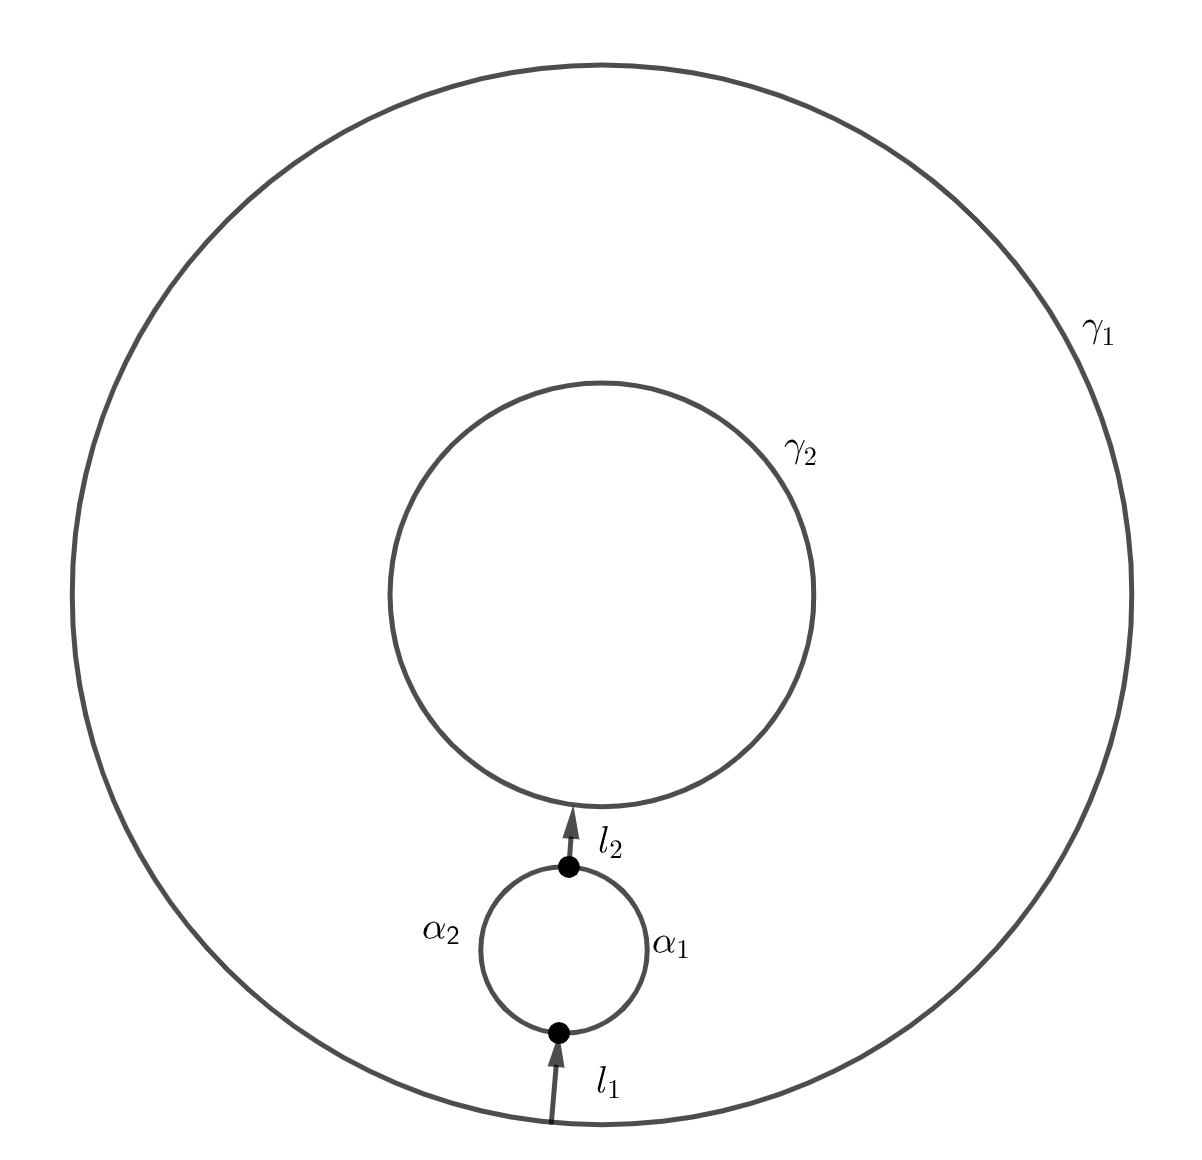
\includegraphics[scale=0.2]{Figure/04_22}
\end{figure}
Il cammino 
$$ \beta=l_1 \star \alpha_1 \star \gamma_2 \star \overline{l_2} \star \alpha_2 \star \overline{l_1}\star \overline{\gamma_1}$$
borda un disco in $B$ dunque \`e omotopicamente banale.\\
Dunque se $f:\, A \to \C$ \`e olomorfa allora la forma $\w=\frac{f(w)}{z-w} \dz $ \`e chiusa  in  $B$  da cui
$$ 0 =\int_\beta \w  = \cancel{\int_{l_1} \w } + \int_{\alpha_1} \w +\int_{\gamma_2} \w + \cancel{\int_{\overline{l_2}}\w} +\int_{\alpha_2} \w + \cancel{\int_{\overline{l_1}} \w} + \int_{\overline{\gamma_1}} \w = \int_{\gamma_2} \w - \int_{\gamma_1} \w +\int_\alpha \w $$
Perci\`o 
$$ \int_{\alpha} \w = \int_{\gamma_1} \w - \int_{\gamma_2} \w $$
Per il primo dei due si fa lo stesso conto fatto per la formula di Cauchy.\\
Lungo $\gamma_1$ abbiamo $\abs{\gamma_1(t)} = r_1>\abs z$.\\
Perci\`o se $w=\gamma_1(t)$ otteniamo 
$$\frac{f(w)}{w-z}  =\frac{f(w)}{w\tonde{1-\frac{z}{w}}} =\frac{f(w)}{w} \cdot \frac{1}{1-\frac{z}{w}} = \frac{f(w)}{w} \sum_{n \geq 0 } \tonde{\frac{z}{w}}^n = \sum_{n \geq 0 }\frac{z^n f(w)}{w^{n+1}}$$
Poich\`e la convergenza di questa serie nella corona $\s{r_2\leq \abs  z \leq r_1}$ \`e normale, dunque uniforme, possiamo scambiare serie e integrale nella seguente catena
$$\int_{\gamma_1} \w  =\int_{\gamma_1} \frac{f(w)}{z-w}\di w = \int_{\gamma_1} \tonde{\sum_{n\geq 0 } \frac{z^n f(w)}{w^{n+1}}} \di w = \sum_{n\geq 0 }z^n \int_{\gamma_1} \frac{f(w)}{w^{n+1}} =\sum_{n \geq 0  } b_n z^n$$
dove abbiamo posto 
$$b_n = \int_{\gamma_1} \frac{f(w)}{w^{n+1}} \di w $$
Notiamo subito che se $\gamma: \, [0,1]\to A$ \`e un qualsiasi cammino omotopicamente equivalente a $\gamma_1$ ovvero  con $I(\gamma, 0)=1$ allora 
$$b_n =\int_{\gamma} \frac{f(w)}{w^{n+1}}\di w $$
infatti $\frac{f(w)}{w^{n+1}}$ \`e chiusa in $A$ ed essere liberamente omotopi in $A$ equivale ad esserlo in $\C 
\setminus \s 0 $ ($\C\setminus \s 0 $ si ritrae per deformazione su $A$) .\\
Andiamo a studiare l'altro integrale: $\int_{\gamma_2} \frac{f(w)}{w-z} \di w $.\\
Se $ w=\gamma_2(t)$, $\abs w < \abs z $ per cui 
$$ \frac{f(w)}{w-z} = -\frac{f(w)}{z-w} = -\frac{f(w)}{z\tonde{1-\frac{w}{z}}} = - \frac{f(w)}{z} \sum_{n \geq 0 } \tonde{\frac{w}{z}}^n  =-\frac{f(w)}{z} \sum_{n\leq 0 } \tonde{\frac{z}{w}}^n  =-\frac{f(w)}{z}\cdot \frac{z}{w} \sum_{n <0} \tonde{\frac{z}{w}}^n  =-\sum_{n <0} \frac{f(w)z^n}{w^{n+1}}$$
Dunque come nello studio precedente
$$ -\int_{\gamma_2} \w = -\int_{\gamma_2} \frac{f(w)}{w-z}\di w  = \int_{\gamma_2} \tonde{\sum_{n<0} \frac{f(w) z^n}{w^{n+1}}} \di w  = \sum_{n<0} z^n \int_{\gamma_2} \frac{f(w)}{w^{n+1}} = \sum_{n<0} b_n z^n$$
dove
$$ b_n =\int_{\gamma_2} \frac{f(w)}{w^{n+1}} \di w =\int_{\gamma} \frac{f(w)}{w^{n+1}} \di w \text{ per ogni } \gamma:\, [0,1]\to A \text{ con } I(\gamma,0)=1$$
Dunque dalla formula integrale di Cauchy, otteniamo 
$$ f(z)= \frac{1}{2\pi i } \int_{\alpha} \frac{f(w)}{w-z} \di w = \frac{1}{2 \pi i }\tonde{\int_{\gamma_1} \w - \int_{\gamma_2} \w } =\frac{1}{2\pi i } \tonde{\sum_{n \geq 0 } b_n z^n + \sum_{n<0} b_n z^n } = \frac{1}{2\pi i } \sum_{n \in \Z} b_n z^n $$
Dunque $f$ ammette uno sviluppo di Laurent 
$$ f(z) = \sum_{n \in \Z} b_n z^n \text{ dove } a_n = \frac{b_n}{2\pi i } =\frac{1}{2\pi i } \int_{\gamma} \frac{f(w)}{w^{n+1}} \di w \text{ per qualsiasi } \gamma \text{ in  } A \text{ con }  I(\gamma,0)=1$$
\end{thm}
\begin{oss}Dalla definizione degli $a_n$ visti sopra si ha (come nel caso gi\`a visto)  $\forall n \in \Z$
$$ \abs{a_n} \leq \frac{M(r)}{r^n} \text{ dove }  M(r) = \sup\s{\abs{f(w)}\, : \, \abs{w} = r}$$
\end{oss}
\begin{cor}Sia $A=\s{\rho_2<\abs z \rho_1}$ e $f:\, A \to \C$ olomorfa.\\
Allora $f=f_1(z) +f_2(z)$ dove le funzioni 
$$ f_1:\, B(0,\rho_1)\to \C$$
$$ f_2:\, \C \setminus \overline{B(0, \rho_2} \to \C$$ 
sono olomorfe.\\
Richiedendo che $\ds \lim_{\abs z \to 0 } \abs{f_2(z)} = 0 $ tale scrittura \`e unica
\proof Essendo $f$ olomorfa sulla corona circolare, ammette un'espansione di Laurent
$$ f(z) =\sum_{n \in \Z} a_n z^n$$
Per l'esistenza poniamo 
$$ f_1(z) = \sum_{n \geq 0 } a_n z^n$$
$$f_2(z) = \sum_{n <0} a_n z^n$$
(tali serie convergono sui rispettivi domini delle funzioni).\\
Mostriamo adesso l'unicit\`a.\\
Se $f(z)=g_1(z) + g_2(z)$ possiamo definire $F:\, \C \to \C$ ponendo 
$$ F(z) =\begin{cases} f_1(z) - g_1(z) \text{ se } \abs z < \rho_1 \\
g_2(z) - f_2(z) \text{ se } \abs{z} > \rho_2  \end{cases}$$
Mostriamo che tale funzione \`e ben definita, da cui segue che \`e olomorfa.\\
Nell'intersezione $\rho_2< \abs z < \rho_1$ abbiamo che 
$$ f_1(z) +f_2(z) = g_1(z) + g_2(z)$$ 
in quanto entrambe coincidono con $f(z)$ per cui 
$$ f_1(z) - g_2(z) = g_1(z) -f_2(z)$$
dunque la funzione $F$ \`e ben definita.\\
Osserviamo $$\lim_{\abs z \to + \infty } F(z) = \lim_{\abs z \to +\infty } g_2(z) - f_2(z) = 0$$ 
dunque 
$F: \, \C \to \C$ \`e olomorfa e limitata, per Louivelle \`e costante.\\
Avendo limite nullo $F$ \`e nulla il che implica che $f_i=g_i$ per $i=1,2$
\endproof
\end{cor}
\newpage
\section{Singolarit\`a }
\begin{defn}Sia $a\in \C$ allora chiamiamo dischi puntati, corone circolari della forma $0< \abs{z-a} < R$ ovvero $B(a,R)\setminus \s a $ dove $R>0$
\end{defn}
\begin{thm}Sia $D\subseteq \C$ aperto e $z_0\in D$.\
Se $f:\, D\setminus \s{z_0} \to \C$ \`e olomorfa, allora
$$ f\text{ si estende ad una funzione olomorfa } g:\, D \to \C \quad \ses \quad f \text{ limitata in un intorno di } z_0$$
\proof $\implica$ Essendo $g$ olomorfa \`e continua, dunque localmente limitata.\\
$\iimplica$ Essendo $f$ limitata in un intorno di $z_0$, esiste $\varepsilon>0$ tale che $B = B(z_0, \varepsilon) \subseteq D$ e 
$$ \abs{f(z)} \leq M \text{ per } z\in B \setminus \s{z_0}$$
Ora $f$ \`e olomorfa in una corona circolare, dunque ammette uno sviluppo di Laurent su $B \setminus \s{z_0}$ ovvero 
$$ f(z) = \sum_{n \in \Z} a_n (z-z_0)^n \text{ per } z\in B \setminus \s{z_0}$$
dunque per quanto abbiamo osservato (dopo il teorema olomorfa implica sviluppo di Laurent) sappiamo 
$$ \abs{a_n} \leq \frac{M}{R^n} \leq \frac{M}{R^n} \text{ per } R<\varepsilon$$
Se $n<0$ allora $\ds \lim_{R\to 0^+} \frac{M}{R^n}=0$ per cui $a_n=0$.\\
Abbiamo dunque notato che la serie di Laurent ha solo termini con esponenti non negativi, dunque $f$ si estende ad una funzione $\overline{f}:\, B(z_0, \varepsilon)\to \C$ olomorfa, possiamo porre
$$ g(z) = \begin{cases}\overline{f}(z) \text{ se } z\in B \\
f(z) \text{ se } z\neq z_0
\end{cases}$$
\end{thm}
\begin{oss}Non basta richiedere che $f$ sia di classe $C^\infty$ infatti la funzione $f(x)=\sin\left(\frac{1}{x}\right)$ \`e limitata ma non si estende in modo continuo in $0$
\end{oss}
\spazio
\begin{defn}Sia $D\subseteq \C$ aperto e $z_0\in D$ e 
sia $f:\, D \setminus \s{z_0}$ olomorfa.\\
Diciamo che $z_0$ \`e una singolarit\`a eliminabile (o rimovibile)  di $f$ se $f$ si estende in modo olomorfo ad una funzione su tutto $D$.\\
Se invece $f$ non si estende in $z_0$  ad una funzione olomorfa, $z_0$ si chiama singolarit\`a isolata
\end{defn}
\begin{defn}Sia $z_0$ una singolarit\`a isolata di $f:\, D\setminus \s{z_0}\to \C$ olomorfa.\\
Sia 
$$ f(z) =\sum_{n \in \Z} a_n (z-z_0)^n$$
uno sviluppo di Laurent in un piccolo disco puntato in $z_0$.\\
Allora $z_0$ si dice
\begin{itemize}
\item polo di ordine $n_0$ se 
$$ \s{ a_n \, \vert \, n< 0 \text{ e } a_n \neq 0 }$$ 
\`e finito e 
$$ n_0 = -\min  \s{ a_n \, \vert \, n< 0 \text{ e } a_n \neq 0 }$$
\item singolarit\`a essenziale se 
$$  \s{ a_n \, \vert \, n< 0 \text{ e } a_n \neq 0 }$$
\`e infinito
\end{itemize}
\begin{oss}Tali definizioni sono valide in quanto lo sviluppo di Laurent di una funzione olomorfa su una corona circolare \`e unico (prossima lezione)
\end{oss}
\end{defn}
\begin{oss}Se $a_n\neq 0$ per qualche $n<0$ allora la singolarit\`a non \`e eliminabile.\\
Sia $a_{n_0} \neq 0$ con $n_0<0$ e consideriamo la funzione $g(z) = f(z)( z-z_0)^{abs{n_0} =1}$.\\
Supponiamo che la funzione $f$ si estenda in $z_0$, dunque anche $g$ si estende.\\
Sia $b_n$ il coefficiente $n$-esimo dello sviluppo di Laurent di $g$, dunque avremmo 
$$ b{-1} = a_{n_0} = \frac{1}{2\pi i } \int_{\gamma} \frac{g(w)}{(w-z_0)^{-1+1}} \di w = \frac{1}{2\pi i } \int_\gamma g(w) \di w =0$$ 
perch\`e $g$ \`e olomorfa in $z_0$.\
\
Abbiamo mostrato che $a_{n_0} = 0 $ ma avevamo supposto $a_{n_0} \neq 0 $\end{oss}
\end{document}